\section{Motivation}
\label{sec:motivation}

\subsection{Threat Model}%
\label{sub:threat_model}

Sultan \etal~\cite{sultan2019_container_security} propose four broad categories of container-related threats. \Cref{fig:threat_model} presents an overview of each category. An application running within a container might attack the container itself, attempting to escape confinement or interfere with the execution of co-located applications running within the same container. Inter-container threats are similarly possible, wherein one container attempts to interfere with or take over another. Since containers share the underlying host operating system, it is also possible for a container to directly attack the host, either by escaping confinement altogether or by launching denial of service or resource consumption attacks. Finally, a malicious or semi-honest host system may attack containers running within it. Researchers have generally recognized that mitigating this fourth category of attack requires the use of hardware security mechanisms \cite{sultan2019_container_security,xin2018_container_security,chen2019_container_dos} such as trusted execution environments or trusted platform modules. Such host-to-container attacks are, therefore, out of scope for this paper.

\begin{figure}[htpb]
  \centering
  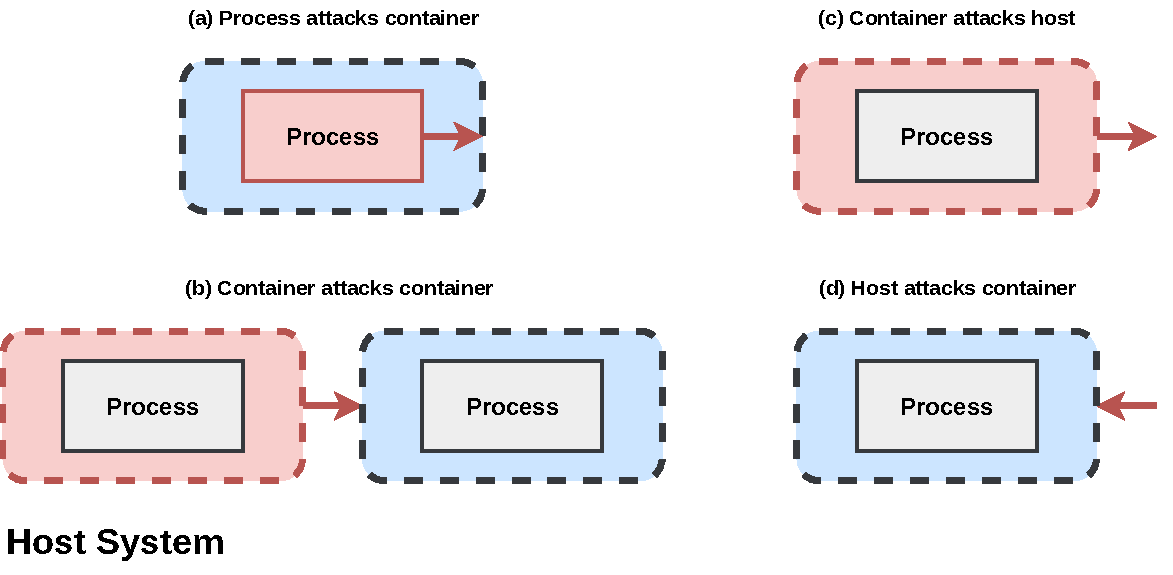
\includegraphics[width=0.8\linewidth]{figs/threat-model.pdf}
  \caption{
    Four categories of container-related attacks \cite{sultan2019_container_security}. \textbf{(a)} A process running within a container attacks the container itself. \textbf{(b)} One container attacks another container. \textbf{(c)} A container attacks the host system. \textbf{(d)} The host system attacks the container. This fourth category of attack is out of scope for this paper.
  }%
  \label{fig:threat_model}
\end{figure}

In this threat model, we consider three broad classes of attack vector, comprised of the containers and the applications that run within them. These attack vectors are described in turn below.
\begin{enumerate}[label=\bfseries AV\arabic*., ref=AV\arabic*, labelindent=1em]
  \item \textsc{Malicious Applications.}
    A malicious application is designed with express malicious intent. Malicious software may actively attempt to subvert other applications, other containers, or the host system itself. This subversion could include privilege escalation attacks on the host system, denial of service attacks on other containers or the host, or the installation of backdoors. A sophisticated attacker could even abuse a malicious application to install a rootkit \cite{beegle2007_rootkit} in the container, on the host system, or in the host's firmware, stealthily gaining permanent and possibly overprivileged access.

  \item \textsc{Semi-Honest Applications.}
    In contrast with malicious applications, semi-honest applications are not necessarily expressly designed with malicious intent and might even be cooperative with other applications or containers. However, the semi-honest application can passively participate in unwanted activity, such as surveillance or consumption of the host's resources.

  \item \textsc{Vulnerable Applications.}
    Vulnerable applications running inside containers may become compromised by attackers, often with the goal of using these applications to orchestrate a more sophisticated attack on other applications running within the same container, other containers, or the host system itself \cite{sultan2019_container_security}. Common vulnerabilities here include code execution vulnerabilities on untrusted input, memory corruption bugs, and privilege escalation vulnerabilities in a container's configuration. Exploitation of kernel-level vulnerabilities are also a concern here, as an attacker can potentially abuse a legitimate application to target vulnerable code paths in the kernel \cite{xin2018_container_security}.
\end{enumerate}

An attacker could have several goals under this threat model. Such goals might include \cite{sultan2019_container_security,xin2018_container_security}:
\begin{enumerate}[label=\bfseries AG\arabic*., ref=AG\arabic*, labelindent=1em]
  \item \textsc{Escalation of Privilege.}
    An attacker that manages to escalate privileges within the context of a container may escape confinement altogether and interfere with the host or with other containers. In the worst case, the attacker may obtain root privileges and establish total control over the host system.

  \item \textsc{Denial of Service.}
    An attacker might abuse a poorly configured container to mount a denial of service attack on the host system or other containers. For instance, an attacker could consume resources on the host system, disable network interfaces, unmount filesystems, or kill other running processes.

  \item \textsc{Remote Code Execution.}
    Remote code execution vulnerabilities could allow an attacker to control a container or, in the worst case, the host itself. Kernelspace code execution vulnerabilities are particularly dangerous, as they can often be used for escalation of privilege, information leakage, or denial of service and affect the entire host system \cite{sultan2019_container_security, xin2018_container_security}.

  \item \textsc{Information Disclosure.}
    An attacker might disclose sensitive information, such as API keys, secret cryptographic keys, passwords, or other sensitive user data. In the worst case, they might be able to disclose information belonging to another container or the host itself.

  \item \textsc{Tampering.}
    An attacker could tamper with other processes running within a container, other containers, or the host itself. Such tampering attacks might include replacing or modifying file systems or data to deliberately induce incorrect computational results \cite{sultan2019_container_security}.

  \item \textsc{Backdoor Establishment.}
    An attacker can establish a backdoor to obtain permanent or semi-permanent access to a container or the host system itself. For instance, an SSH backdoor (e.g.~installing an attacker-controlled public key into SSH's list of authorized keys) can enable persistent network intrusions on the host system. In the worst case, this might involve installing a rootkit \cite{beegle2007_rootkit} in the host operating system to enable stealthy, overprivileged access.
\end{enumerate}

Since containers are often co-located in large-scale, multi-tenant systems such as the cloud \cite{sultan2019_container_security}, the potential for exploitation or abuse by foreign threat actors is exacerbated. Thus, container management systems must enforce least-privilege on containers to prevent such exploitation from negatively impacting the rest of the system. A secure container management system with sensible defaults and strong protection mechanisms would defeat most, if not all, of the attacks outlined above.

\subsection{The Quest for Secure Containers}%
\label{sub:secure_containers}

Sultan \etal~ cite container security issues as the primary factor inhibiting their widespread adoption \cite{sultan2019_container_security}. In existing container management systems, least-privilege is often treated as a secondary goal. Instead, light-weight virtualization, dependency management, convenience, and environmental reproducibility are prioritized. For instance, Docker \cite{docker,sultan2019_container_security} provides an overly permissive default security policy, enabling the use of several dangerous system calls and POSIX capabilities. Extra protection, such as the system call restrictions offered by its default seccomp and AppArmor policies, is considered opt-in rather than opt-out \cite{docker,sultan2019_container_security}. Further, in an environment where running AppArmor is not an option, Docker must forgo the protection offered by its AppArmor policy altogether.

Other container security issues arise when attackers can bypass protection mechanisms altogether. For instance, code execution attacks in kernelspace can be mounted by exploiting vulnerabilities in the kernel's API and bypassing memory protection mechanisms. Depending on the attack, the interfaces required to mount such an exploit successfully may not even be gated by a container security mechanism. Such exploits effectively reduce security to that of a process running directly on the host system. While these attacks may be difficult to mount in practice, they still merit consideration.

Unlike full hardware virtualization under a hypervisor, containers must share the underlying host operating system kernel and resources. In practice, this means that their attack surface is fundamentally larger than that of a virtual machine. If we are to strive for genuinely secure containers, we must seek to minimize this attack surface as much as possible. This means that we need to build containers to be secure from the ground-up, prioritizing least-privilege over all other goals.
